\documentclass[12pt,a4paper]{article}
\usepackage[T1]{fontenc}
\usepackage[utf8]{inputenc}
\usepackage{amsmath,amsfonts,amssymb,bm}
\usepackage{tikz}

\begin{document}

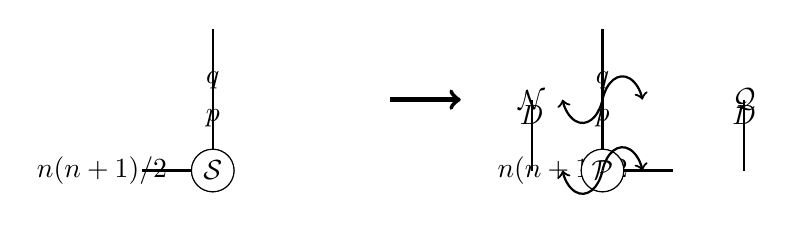
\begin{tikzpicture}[scale=0.9]
\draw[thick] (1,-3) -- node[below] {$p$} (1,-1);
\draw[thick] (1,-3) -- node[left] {$n(n+1)/2$} (0,-3);
\draw[thick] (1,-3) -- node[above] {$q$} (1,-1);
\draw[fill=white](1,-3) circle (.3);
\draw[fill=white](1,-3) circle (.3);
\node at (1,-3) {\color{black}{$\mathcal{S}$}};
\draw[ultra thick,->] (3.5,-2) -- (4.5,-2);
\draw[thick] (6.5,-3) -- node[below] {$p$} (6.5,-1);
\draw[thick] (6.5,-3) -- node[left] {$n(n+1)/2$} (7.5,-3);
\draw[thick] (6.5,-3) -- node[above] {$q$} (6.5,-1);
\draw[fill=white](6.5,-3) circle (.3);
\draw[fill=white](6.5,-3) circle (.3);
\node at (6.5,-3) {\color{black}{$\mathcal{P}$}};
\draw[thick,->] (6.5,-2) arc (-20:-160:.3cm and .5cm);
\draw[thick,->] (6.5,-2) arc (160:20:.3cm and .5cm);
\draw[thick] (5.5,-3) -- node[above] {$D$} (5.5,-2);
\node at (5.5,-2) {\color{black}{$\mathcal{N}$}};
\draw[thick,->] (6.5,-3) arc (-20:-160:.3cm and .5cm);
\draw[thick,->] (6.5,-3) arc (160:20:.3cm and .5cm);
\draw[thick] (8.5,-3) -- node[above] {$D$} (8.5,-2);
\node at (8.5,-2) {\color{black}{$\mathcal{Q}$}};
\end{tikzpicture}

\end{document}